\documentclass{ctexart}
\usepackage[utf8]{inputenc}
\usepackage{graphicx}
\usepackage{tikz}
\usetikzlibrary{shapes,arrows}


\title{作业2: Binary Search Tree}
\author{陈科辉 Keiver Pabula}
\date{19 Octobe,2022}
\begin{document}
\maketitle

作业2:二叉搜索排序算法。
\section{设计思路}
根据老师所发的头文件添加两种排序函数,一个是先乱序再排序;另一个则是直接排序\\
1. 创建相应的头文件\\
2. 添加sortTree用于有序的打印树\\
3. 在main.cpp中添加BSTSorting制作一个函数,在这个模板函数中,应用传入的数组,并传入模板中;先将异常情况排除;如果$\_mode=0$则正常运行,如果$\_mode=1$则先乱序用$random\_shuffle$\\
4. 生成树,然后再排序; 打印排序前后的tree,和所用的时间\\
5. 函数中使用clock()来计算排序时间,并求出其效率\\
6. 设计主函数:主函数只要用于输入test几次,数组的size(大小)和排序的模式。注意数组的内容是由size所固定的,数组的元素是由0-size这个方法来得到的。\\
7. debuging测试\\
8. 得到结果\\
9. 制作报告\\


\section{测试说明}
输出的内容:\\
2次测试分别是当它是模式0和1时,100个数据的情况:
\begin{center}
  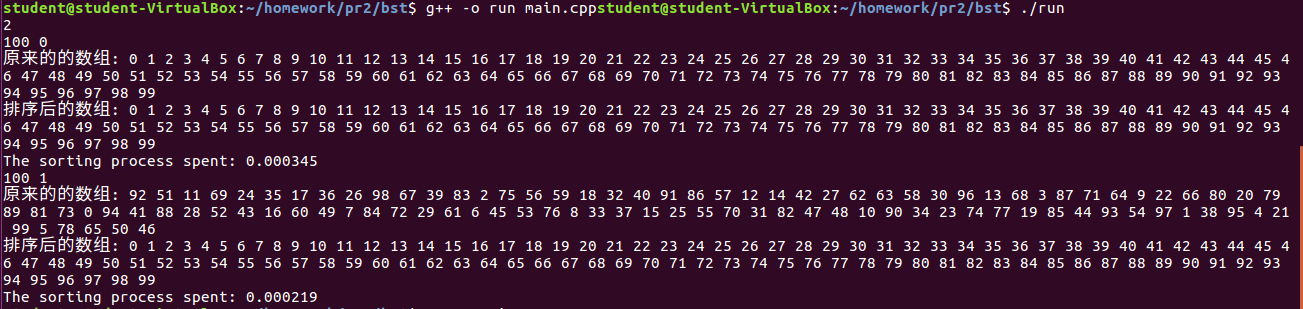
\includegraphics[scale=0.5]{ss1.png}
\end{center}
4次测试分别是当它是模式0和1时,1000和10000个数据的情况:
\begin{center}
  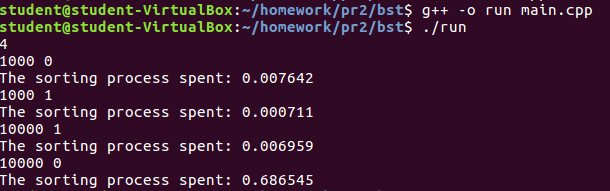
\includegraphics[scale=0.5]{ss2.png}
\end{center}
1次测试,如果模式错误自动退出:
\begin{center}
  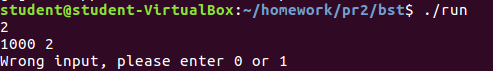
\includegraphics[scale=0.5]{ss3.png}
\end{center}
可以看到排序一切正常,且可以得到他们各自的效率
但是可以看到他们的效率并不稳定:
\begin{center}
  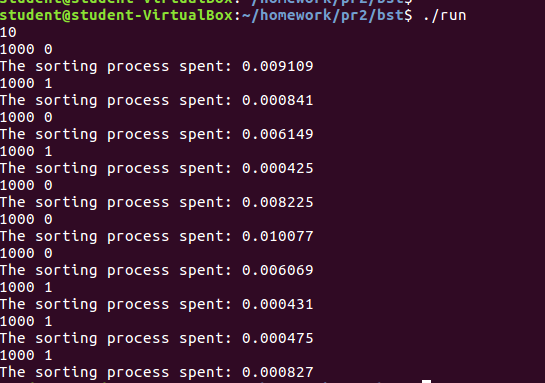
\includegraphics[scale=0.5]{ss4.png}
\end{center}

\end{document}
